\section{Experiment evolution graphs}\label{app:evolution}

Figure~\ref{fig:2} condenses the search to its 51 turning points. The agent maintained the
complete graph, one node per registered experiment and one edge per dependency, and a script
renders it as Mermaid flowcharts and SVG. Three of those renderings are reproduced here
unchanged. Figure~\ref{fig:evo-full} is the complete graph as it stood on 2026-10-13 (snapshot
\texttt{653ceb9}, 207 of the 231 registered experiments; the later T = 4 verification runs are in
Figure~\ref{fig:evo-t4}). It is a map rather than a figure to read on paper: at page size the
node text is about 1 pt high, but the figure is vector and every node is legible when the PDF is
zoomed. The frame times printed in its nodes are HLS-estimated cycles at a 100 MHz reference
clock, which is the basis the agent used to compare designs at the screening gate; they are not
the routed or on-board figures of Table~\ref{tab:22}. Figures~\ref{fig:evo-branches} and
\ref{fig:evo-t4} are two of the seven per-phase views generated from
\texttt{experiments/graph.json} by the script \texttt{evolution\_graph.cjs} of the skill in
Appendix~\ref{app:skill}: the architecture branches that were measured against the mainline and
mostly rejected, and the final workstream that led to the selected design. In every node of the
phase views the first line is the experiment ID and title, the second the one change it makes
relative to its control, the third the primary metric at the evidence level reached (bold where
it is comparable), and the last line the reason it failed a gate ($\times$) or the caveat that goes
with a pass ($!$). Solid edges are design lineage, dashed edges are evidence, control or
verification relations; green nodes passed with a comparable number, red nodes failed a gate,
and the star marks the selected design.

\begin{landscape}
\begin{figure}[p]
\centering
\includegraphics[width=\linewidth,height=0.9\textheight,keepaspectratio]{figures/evolution/full.pdf}
\caption{The complete experiment graph on 2026-10-13: 207 experiments and 217 main
optimisation links, laid out left to right in time. Series E (baseline, precision, directives,
streaming sweeps), F (continuous direct-convolution mainline), P (packing), W (Winograd), G
(scatter), S (tiling and DDR) and C (combinations). Green: passed its stage with a comparable
frame time; amber: HLS timing warning; red: a specific failure, stated in the node; grey:
auxiliary; faded: failed or unrun. Frame times are HLS estimates at 100 MHz. The legend in the
top-left corner is part of the rendering. Zoom in to read.}
\label{fig:evo-full}
\end{figure}
\end{landscape}

% The other five phase views (baseline, stream, mainline, winograd, physical) are rendered to
% figures/evolution/*.pdf as well; uncomment a block below to include one.

% \begin{figure}[p]
% \centering
% 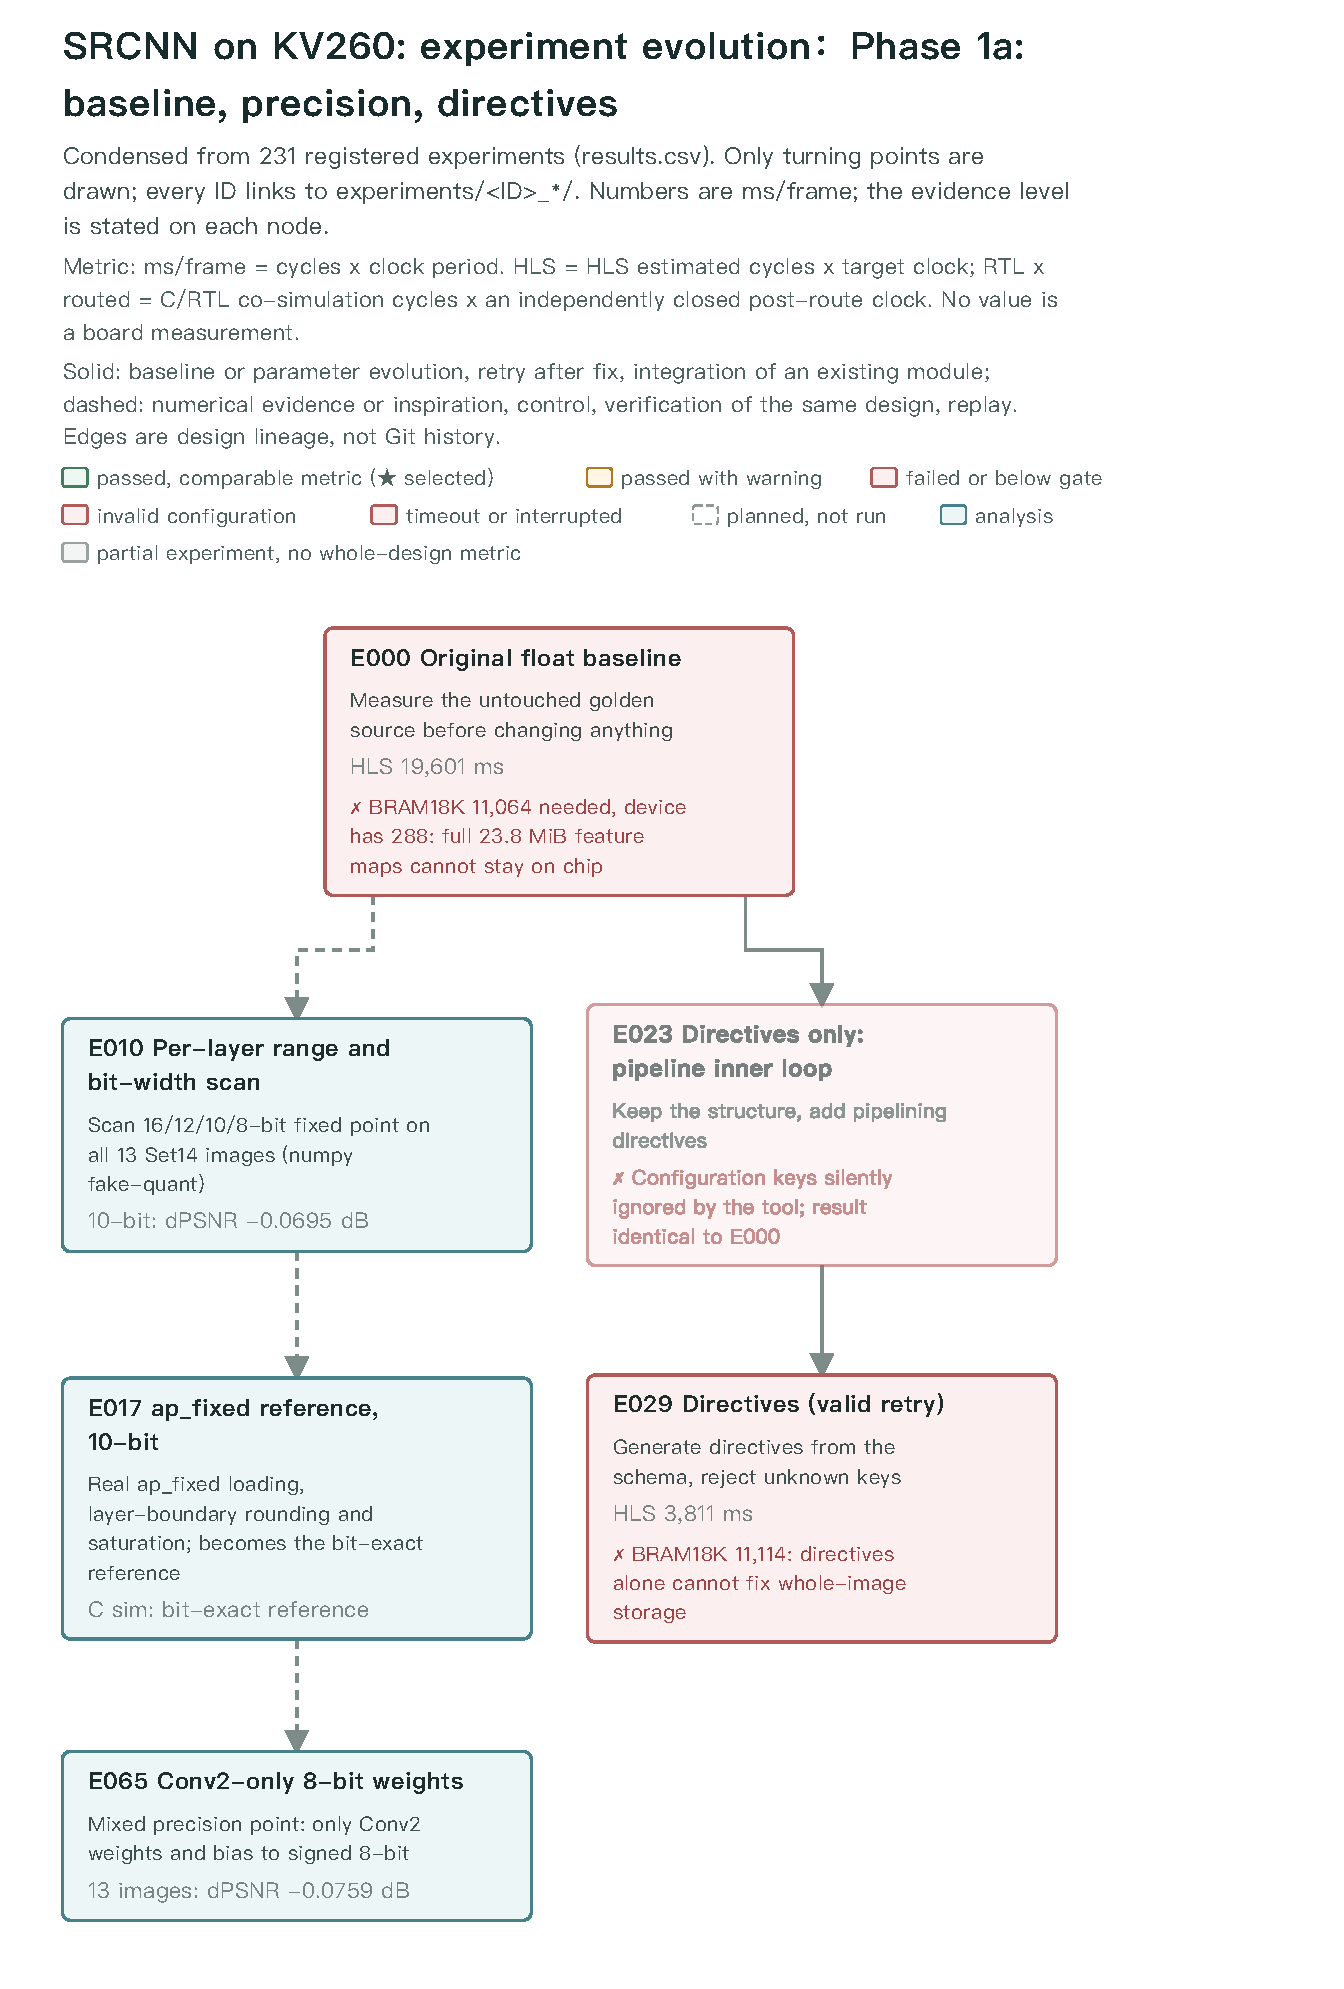
\includegraphics[width=\linewidth,height=0.93\textheight,keepaspectratio]{figures/evolution/baseline.pdf}
% \caption{Phase 1a: baseline, precision and directives. The original float source (E000), the
% precision scan that fixed 10-bit weights and activations (E010), the bit-exact
% \texttt{ap\_fixed} reference (E017) and the directive-only attempts that showed the original
% code cannot fit regardless of pragmas (E020 to E032).}
% \label{fig:evo-baseline}
% \end{figure}

% \begin{figure}[p]
% \centering
% 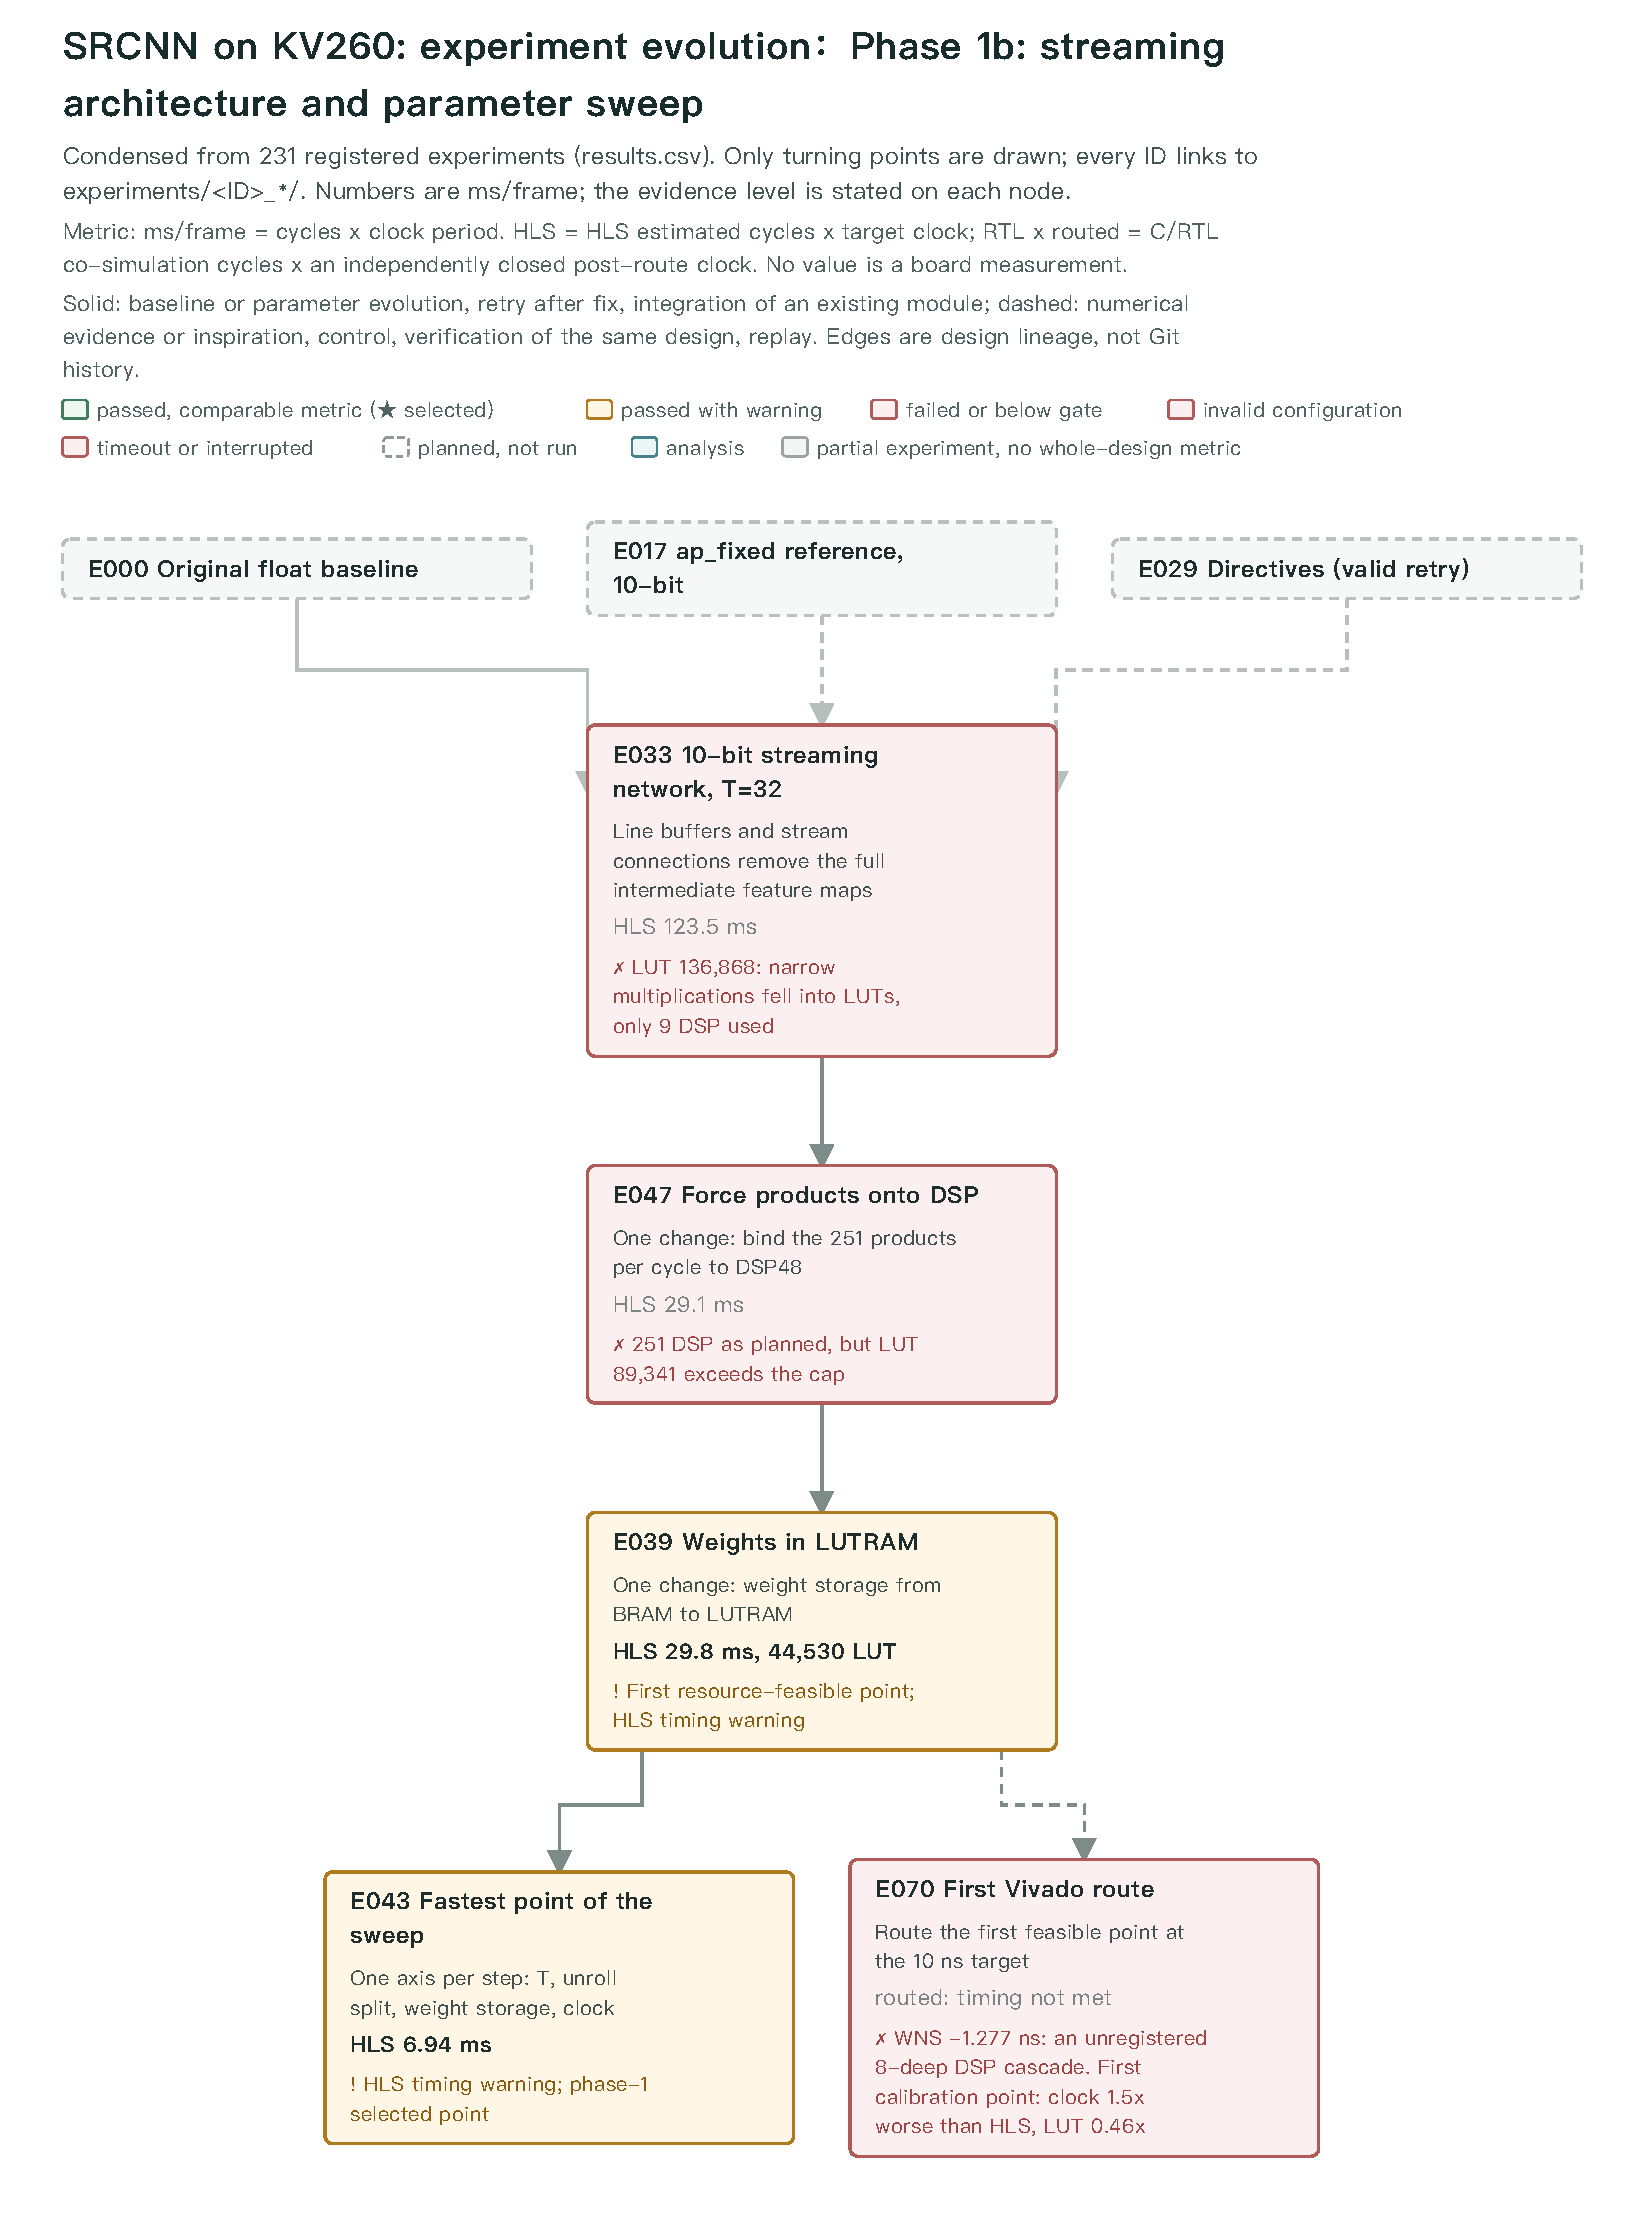
\includegraphics[width=\linewidth,height=0.93\textheight,keepaspectratio]{figures/evolution/stream.pdf}
% \caption{Phase 1b: streaming architecture and parameter sweep. Line buffers and stream
% connections replace the full intermediate feature maps (E033), the products are bound to DSPs
% (E047), the weights move to LUTRAM (E039), and the fold and clock target are swept (E043).}
% \label{fig:evo-stream}
% \end{figure}

% \begin{figure}[p]
% \centering
% 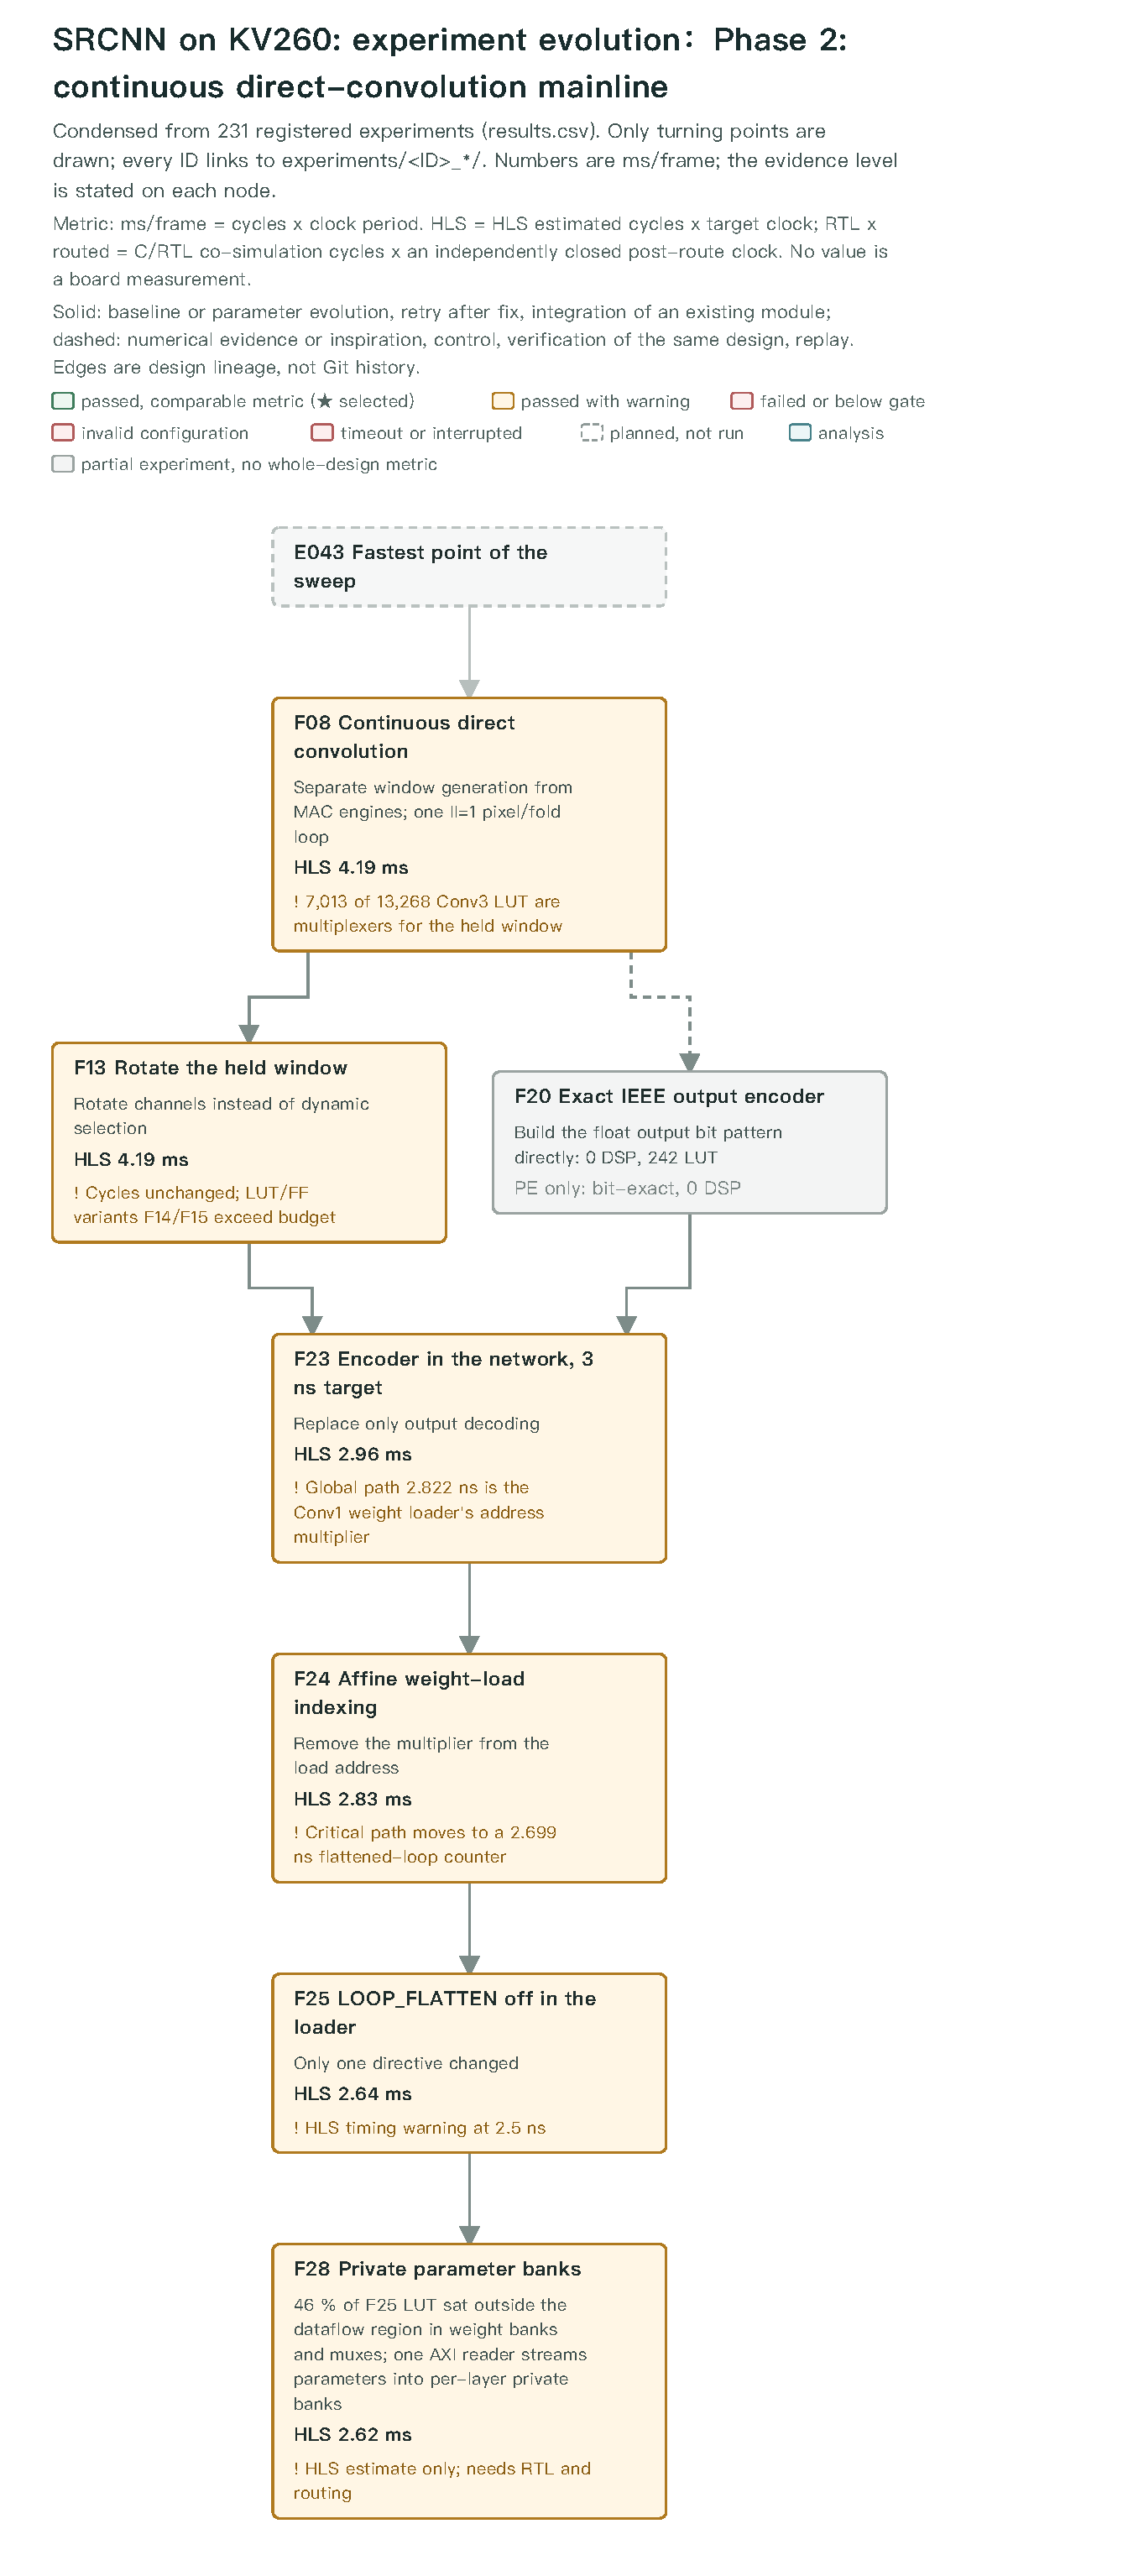
\includegraphics[width=\linewidth,height=0.93\textheight,keepaspectratio]{figures/evolution/mainline.pdf}
% \caption{Phase 2: the continuous direct-convolution mainline. Window generation is separated
% from the MAC engines (F08), the window multiplexers are removed (F13), the output encoder is
% made exact (F20), and the parameter loader is moved off the critical path (F23 to F28).}
% \label{fig:evo-mainline}
% \end{figure}

\begin{figure}[p]
\centering
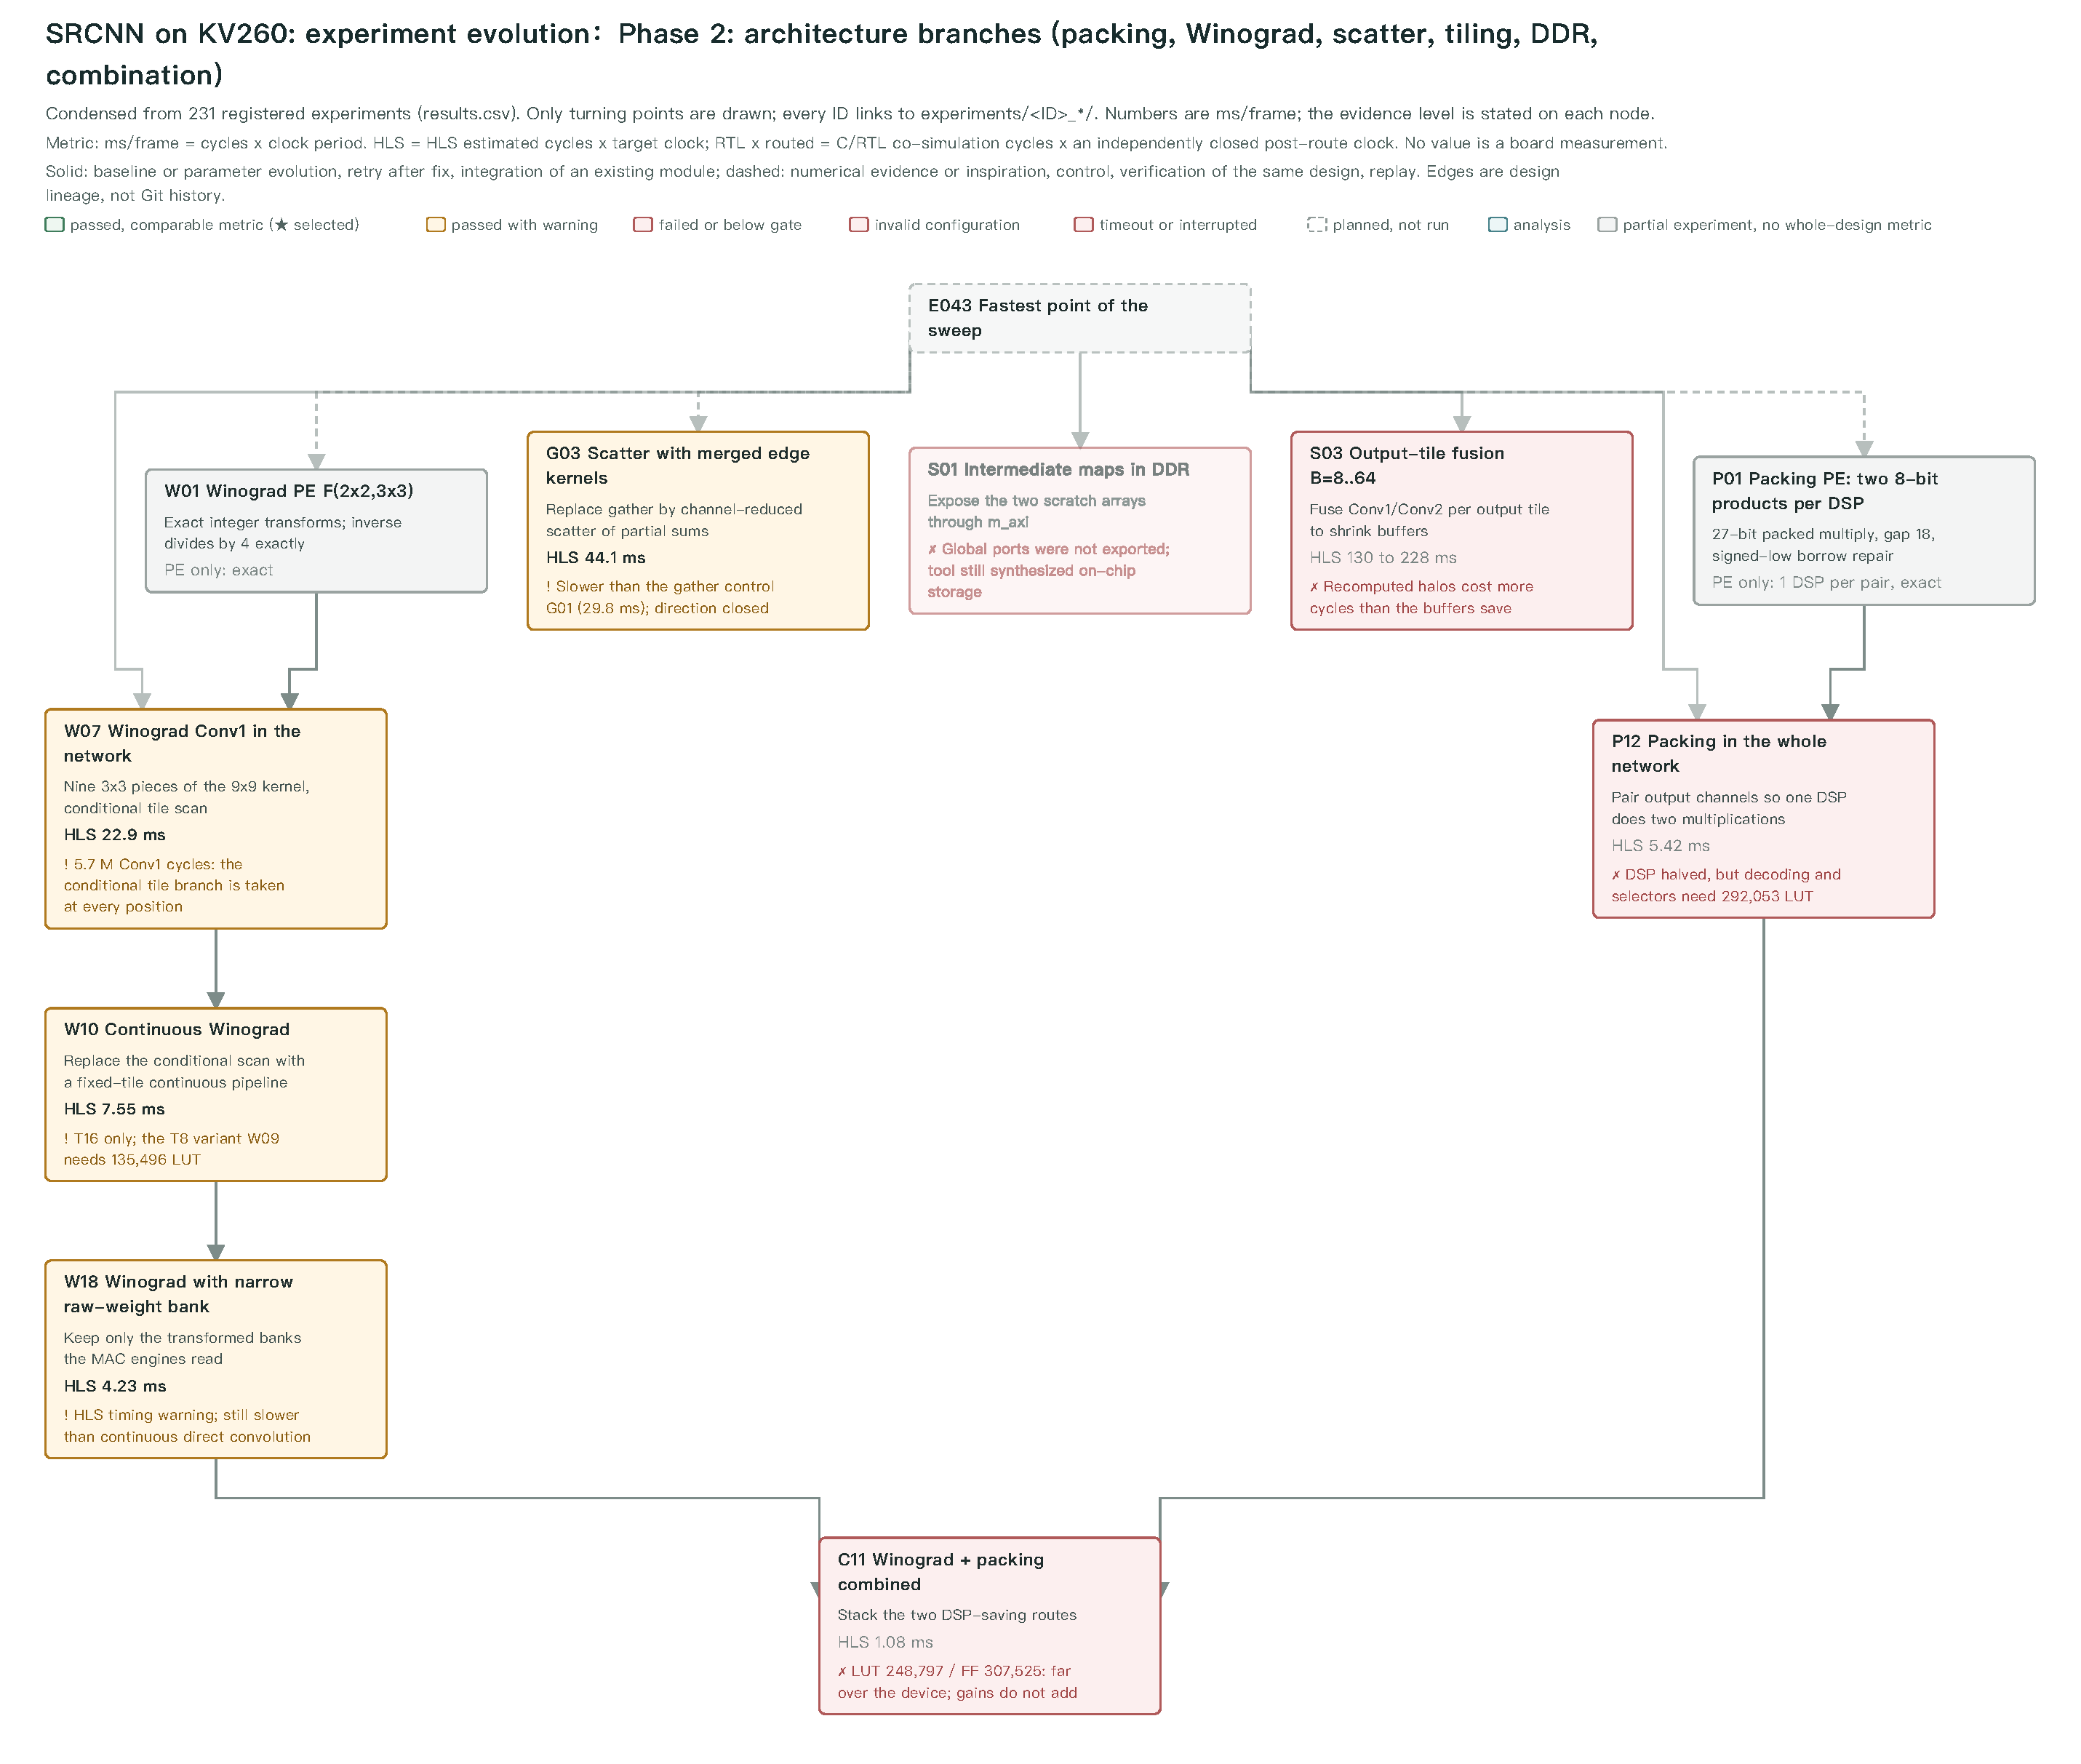
\includegraphics[width=\linewidth,height=0.93\textheight,keepaspectratio]{figures/evolution/branches.pdf}
\caption{Phase 2: architecture branches explored against the mainline: DSP packing (P
series), Winograd (W series), Conv3 scatter (G series), tile fusion and DDR scratch buffers (S
series) and their first combinations (C series).}
\label{fig:evo-branches}
\end{figure}

% \begin{figure}[p]
% \centering
% 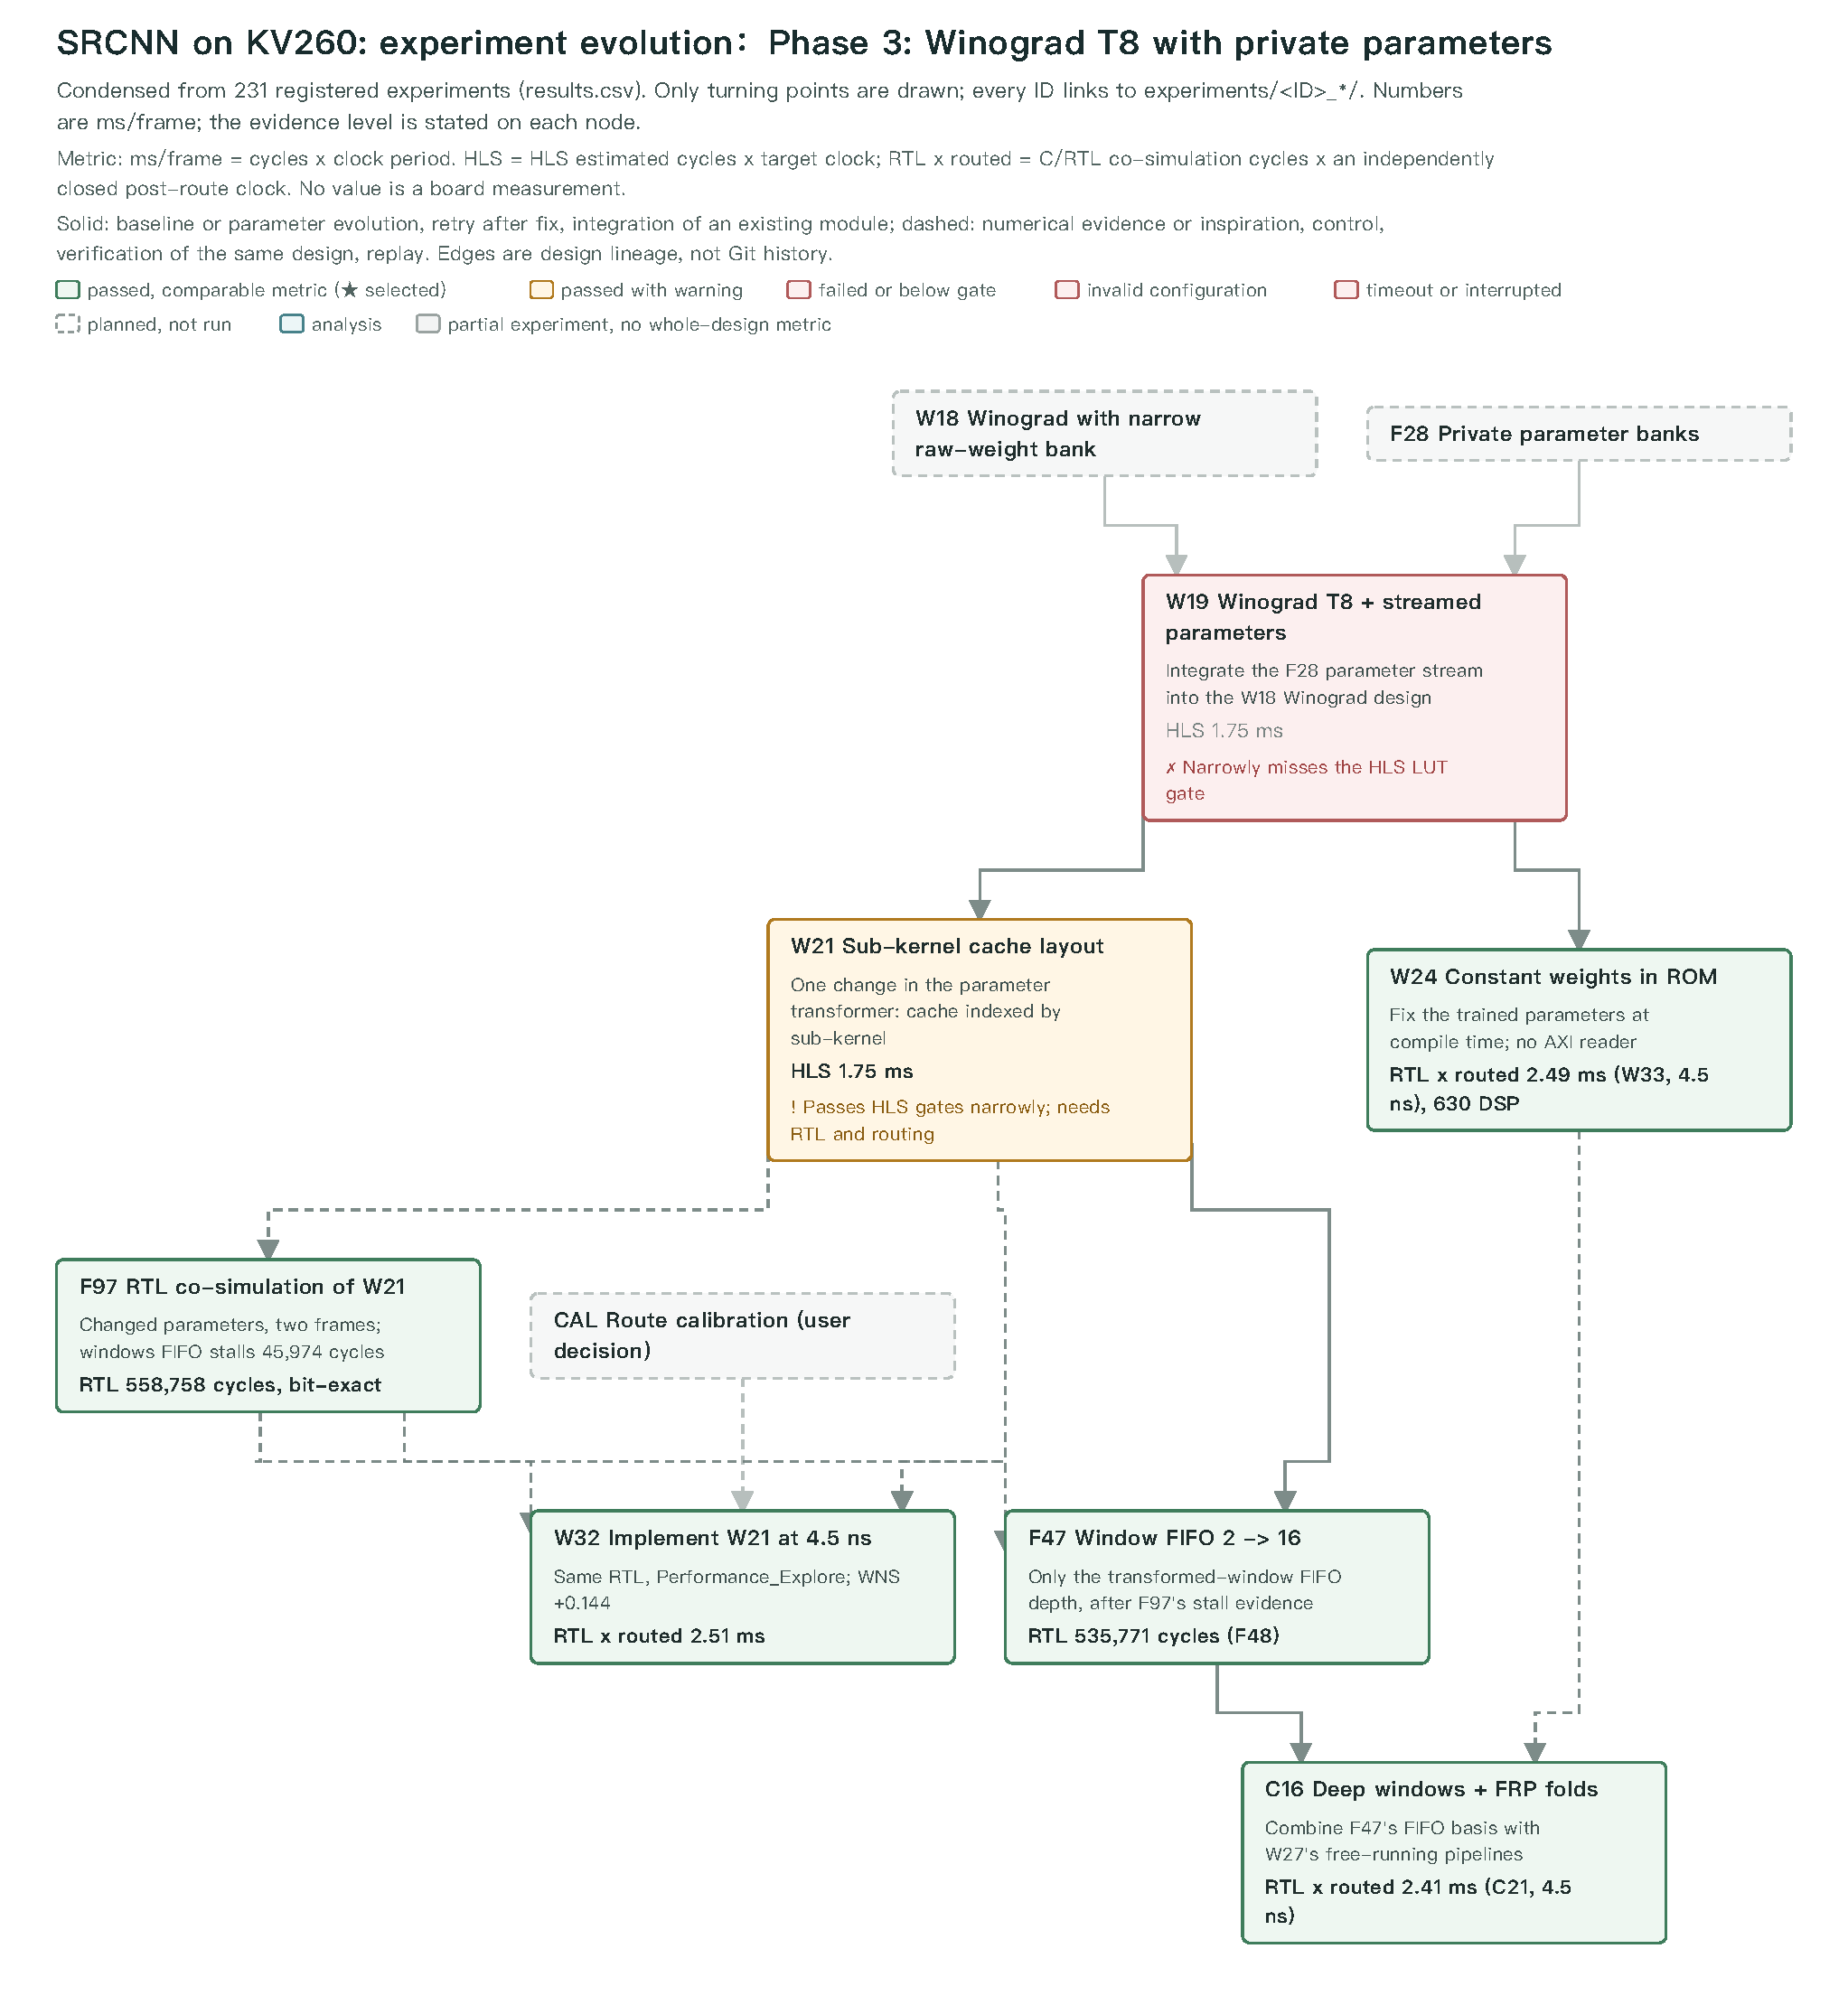
\includegraphics[width=\linewidth,height=0.93\textheight,keepaspectratio]{figures/evolution/winograd.pdf}
% \caption{Phase 3: Winograd at T = 8 with private parameters. The streamed-parameter loader is
% integrated into the Winograd design (W19 to W21), co-simulated (F97) and routed (W32); the
% window-FIFO stall found in F97 leads to F47.}
% \label{fig:evo-winograd}
% \end{figure}

% \begin{figure}[p]
% \centering
% 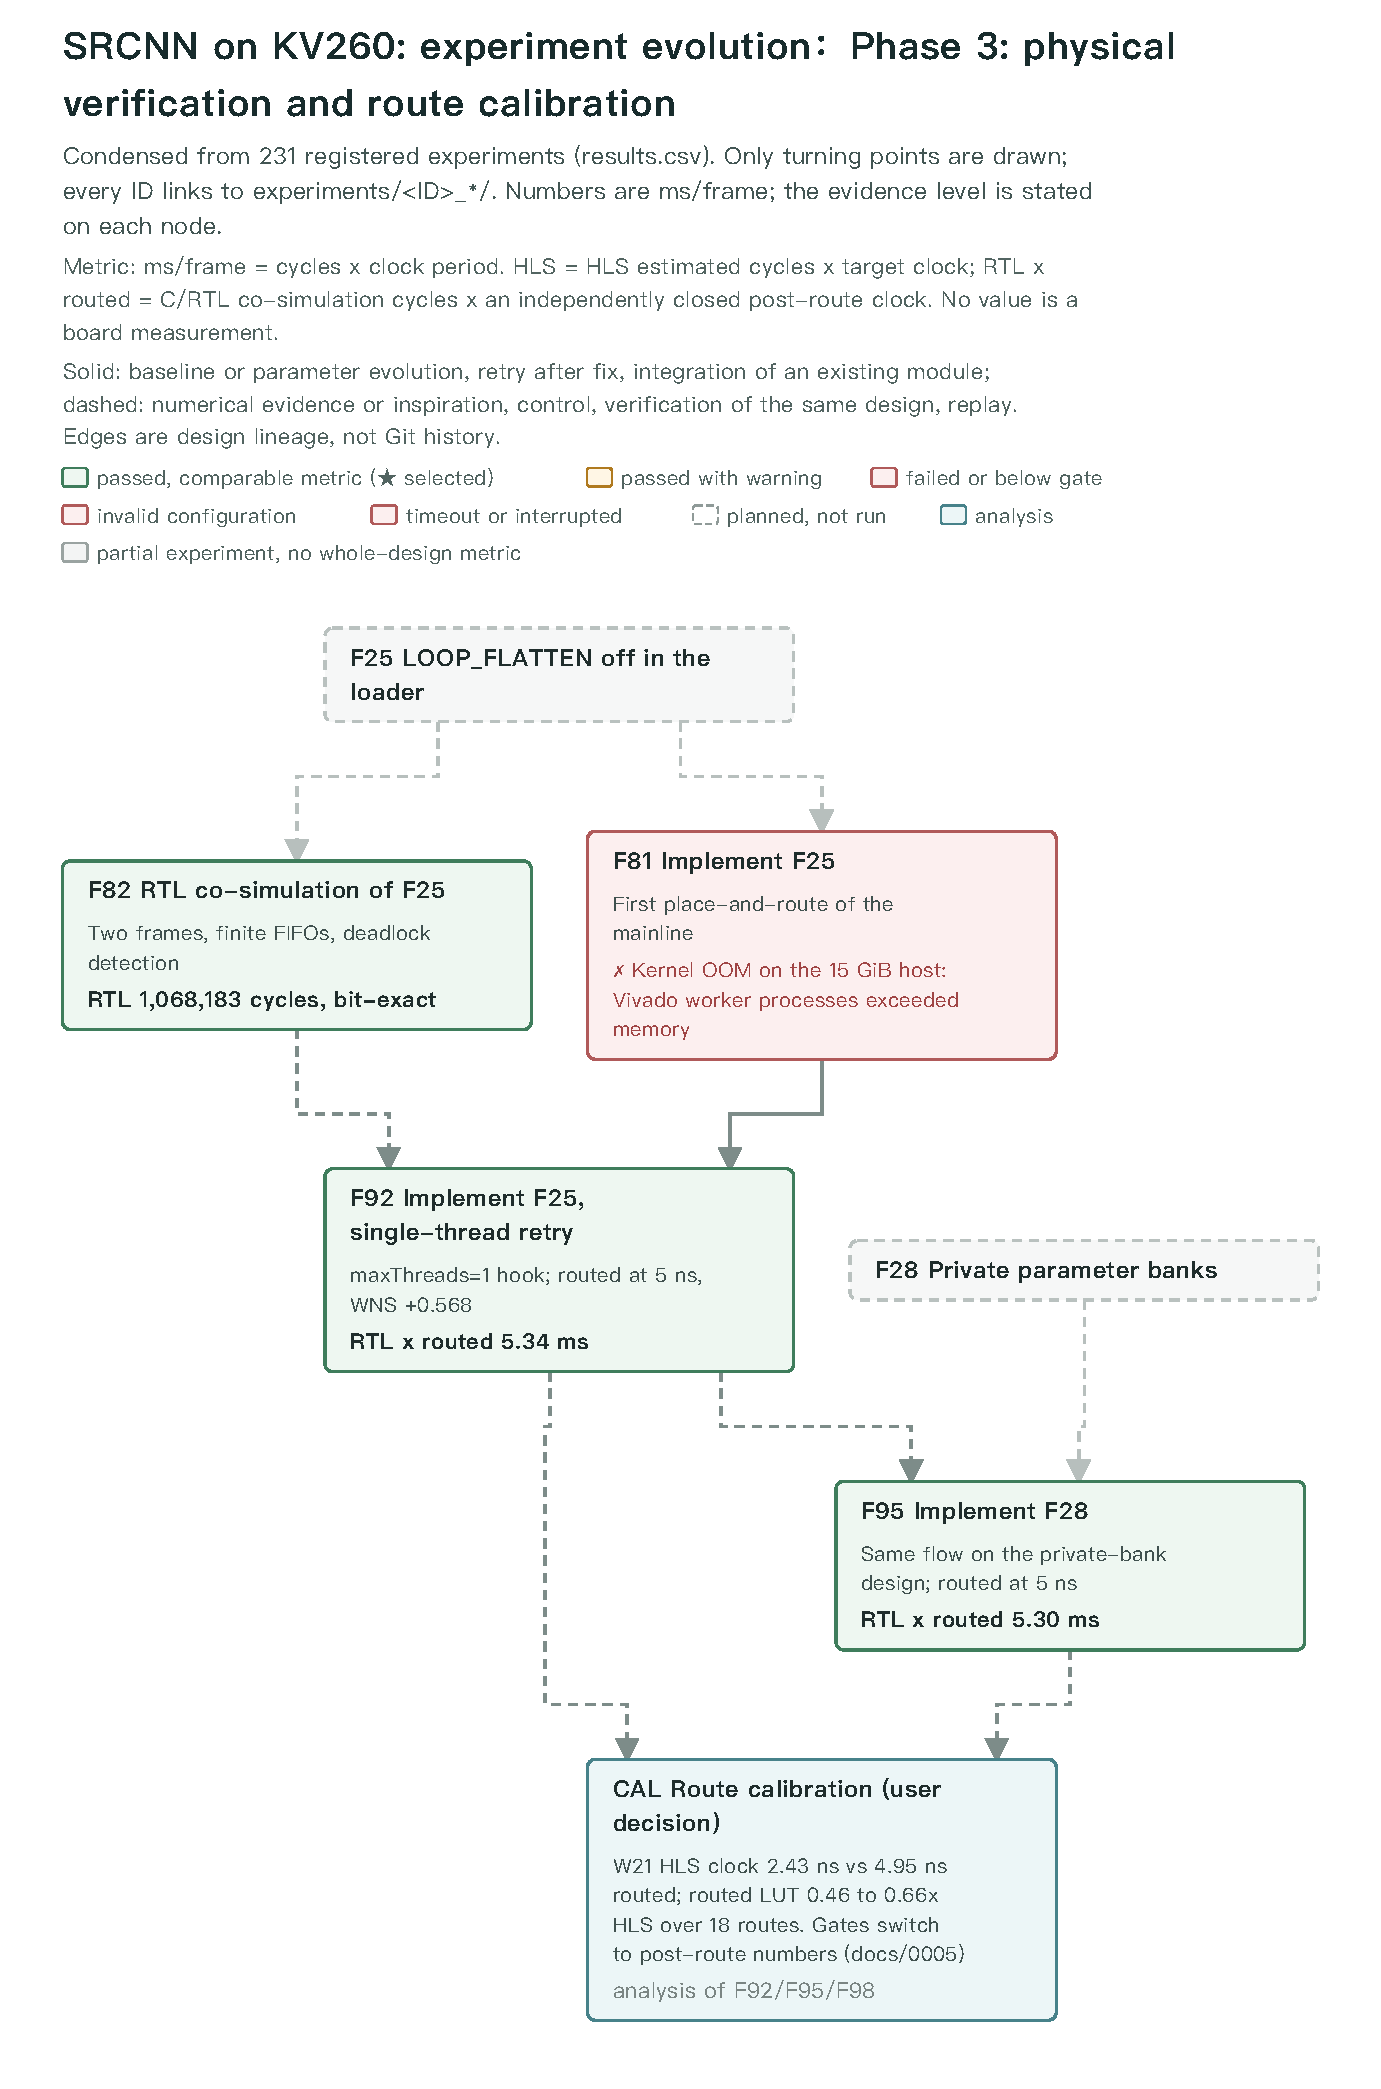
\includegraphics[width=\linewidth,height=0.93\textheight,keepaspectratio]{figures/evolution/physical.pdf}
% \caption{Phase 3: physical verification and route calibration. The first implementations of
% the mainline (F81, F92), the out-of-memory failures that set the host policy, and the routed
% results whose comparison with the HLS estimates changed the gates on 2026-10-12.}
% \label{fig:evo-physical}
% \end{figure}

\begin{figure}[p]
\centering
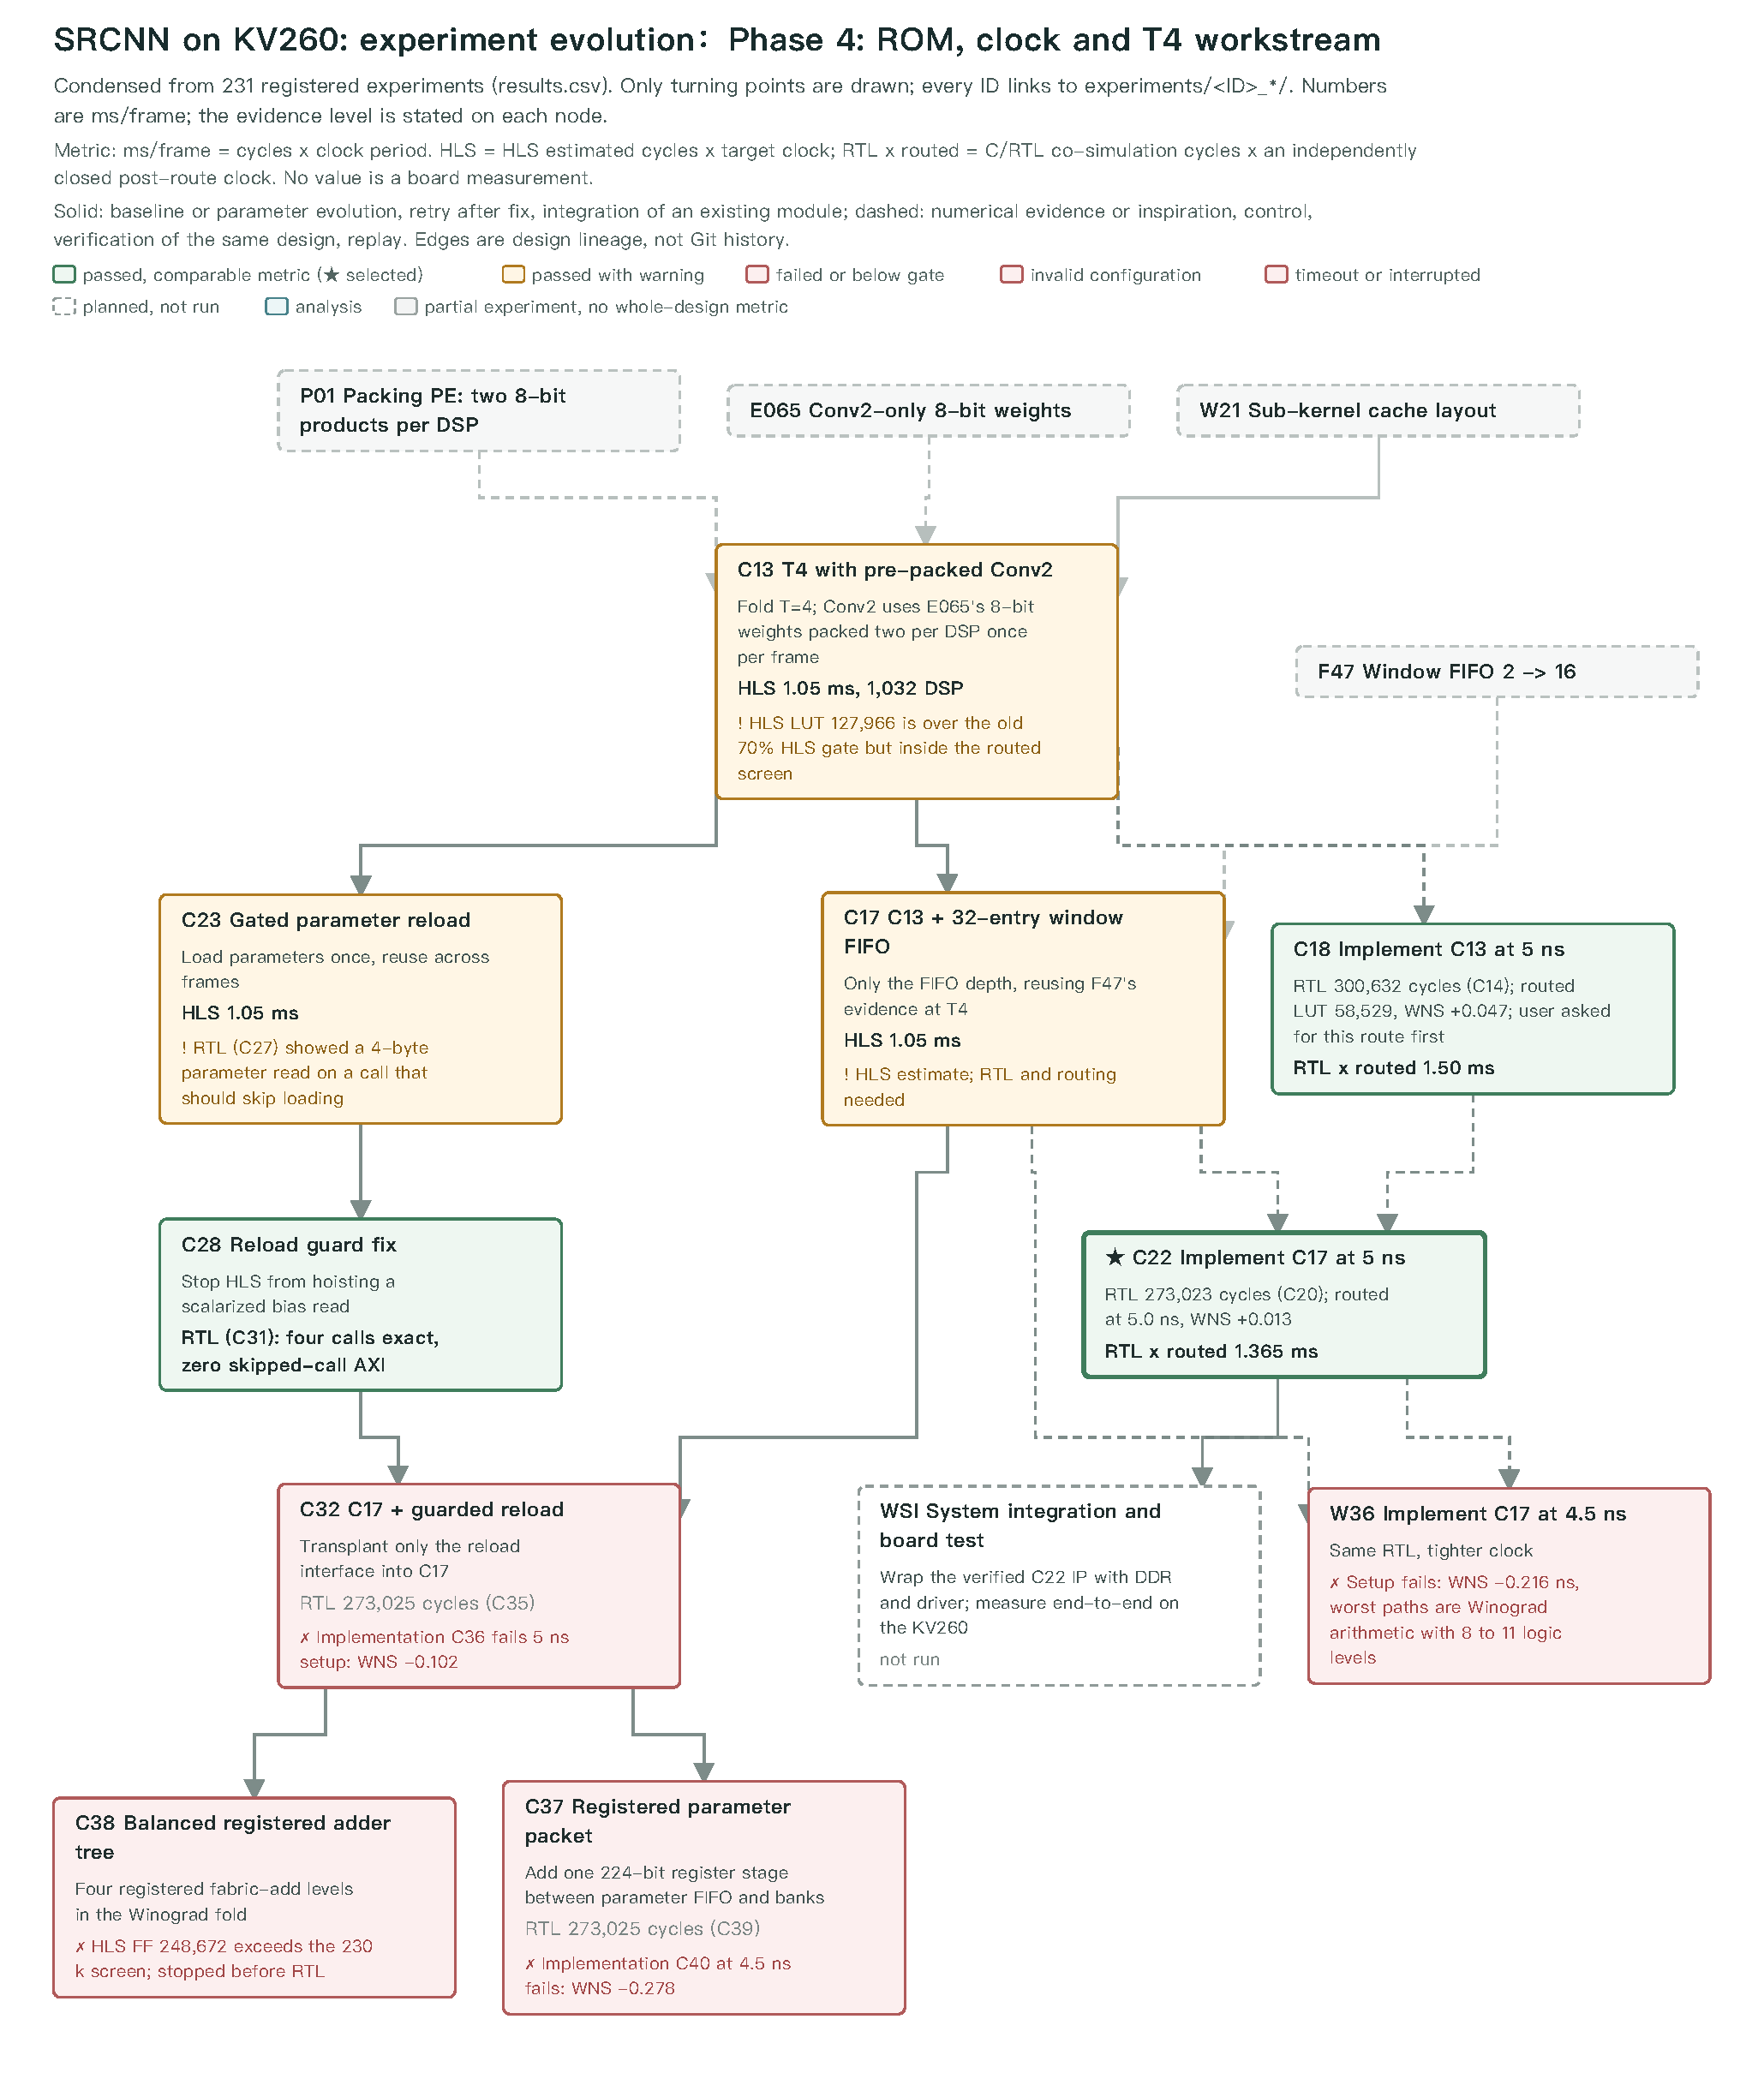
\includegraphics[width=\linewidth,height=0.93\textheight,keepaspectratio]{figures/evolution/t4.pdf}
\caption{Phase 4: ROM parameters, clock and the T = 4 workstream. The pre-packed Conv2
weights make T = 4 fit (C13), the window FIFO is deepened (C17), and the design is
co-simulated (C20) and routed (C18, C22); the attempts at 4.5 ns (W36, C36, C40) fail timing in
the Winograd arithmetic.}
\label{fig:evo-t4}
\end{figure}
